\section{Performance Analysis and Blockchain Related Issues}
\label{sec-performance}

In this Section, we evaluate the performance of the protocol presented above. A proof of concept has been designed using the Ethereum platform and can be found on a GitHub repository [\url{https://github.com/lepilotedef22/anonymous-sealed-bid-auction}]. In order to run the protocol on a full blockchain network, the software \textit{Ganache} (\url{https://www.trufflesuite.com/ganache}) has been used. It allows to simulate an arbitrary Ethereum network. At the time of the writing of this paper, November 30th, 2020, the exchange value of the ether is 589 US dollars and the gas cost is 20 GWei. The gas and US dollar costs of the functions used during the protocol can be found in Table \ref{tab:gas_cost}.
\begin{table}[h]
    \centering
    \csvautotabular{src/price.csv}
    \caption{Gas cost and US dollar cost of the Smart Contract functions called during the execution of the protocol, as of November 30th, 2020.}
    \label{tab:gas_cost}
\end{table}
The auction contract code is written in Solidity language and then compiled to EVM byte code and replicated to Ethereum nodes. The smart contract deployment is one of the most expensive tasks (1861811 gas units) but since this should be executed only once and can then be reused arbitrarily many times, this is an acceptable overhead. The cost of the function placeBid grows linearly with the number of bidders. This is due to the fact that it takes as an input a ring signature, as well as the ring of users itself, which are both proportional to the number of bidders. This is a practical limitation because if a number of bidders above 15 is reached, it will lead to a gas limit exception. However, a simple solution would be to only store a hash of this data on chain and rely on other off-chain resources, such as for example \gls{ipfs} or Swarm, to actually access the data. More sophisticated solutions will be investigated in future work.

At the current stage of development, the \gls{zkp} is still a missing feature. However, it is expected that the overhead linked to this part of the protocol should be close to that of the auction protocol presented by Galal and Youssef\cite{galal2018succinctly}, since our \textsc{VerifiableAuction} algorithm is similar to the one they present. Our new scheme exhibits a major improvement compared to theirs since it enables the bidders to maintain their anonymity by using a \gls{dvrs} approach. This feature requires a maximum of three interactions with the Smart Contract (bid commitment, bid opening and identity opening for the winning bidder), whereas only two are needed in Galal and Youssef's protocol. 

While comparing our proposed work with \cite{galal2018verifiable}, keeping the same number of ten bidders and same blockchain platform, we demonstrate that the Smart Contract deployment cost of our protocol saves 40\%, with respect to deployment cost of 3131261 gas units in~\cite{galal2018verifiable}. Also, other functions such as openBid, announceWinningCommitment and withdrawDeposit consume less gas while placeBid is marginally more expensive in our case. Therefore we conclude that our proposed protocol is more efficient with additional features.

In figure \ref{fig:time}, the auction time as function of the number of bidders taking part to the auction is displayed. This time grows monotonically with the number of bidders. This can be explained by the fact that the rings formed in order to perform the ring signature that ensures anonymity is built by selecting a random number of parties among the bidders. Therefore, the more bidders, the larger the rings on average, and the longer the computations involving them, as indicated above.

\begin{figure}
    \centering
    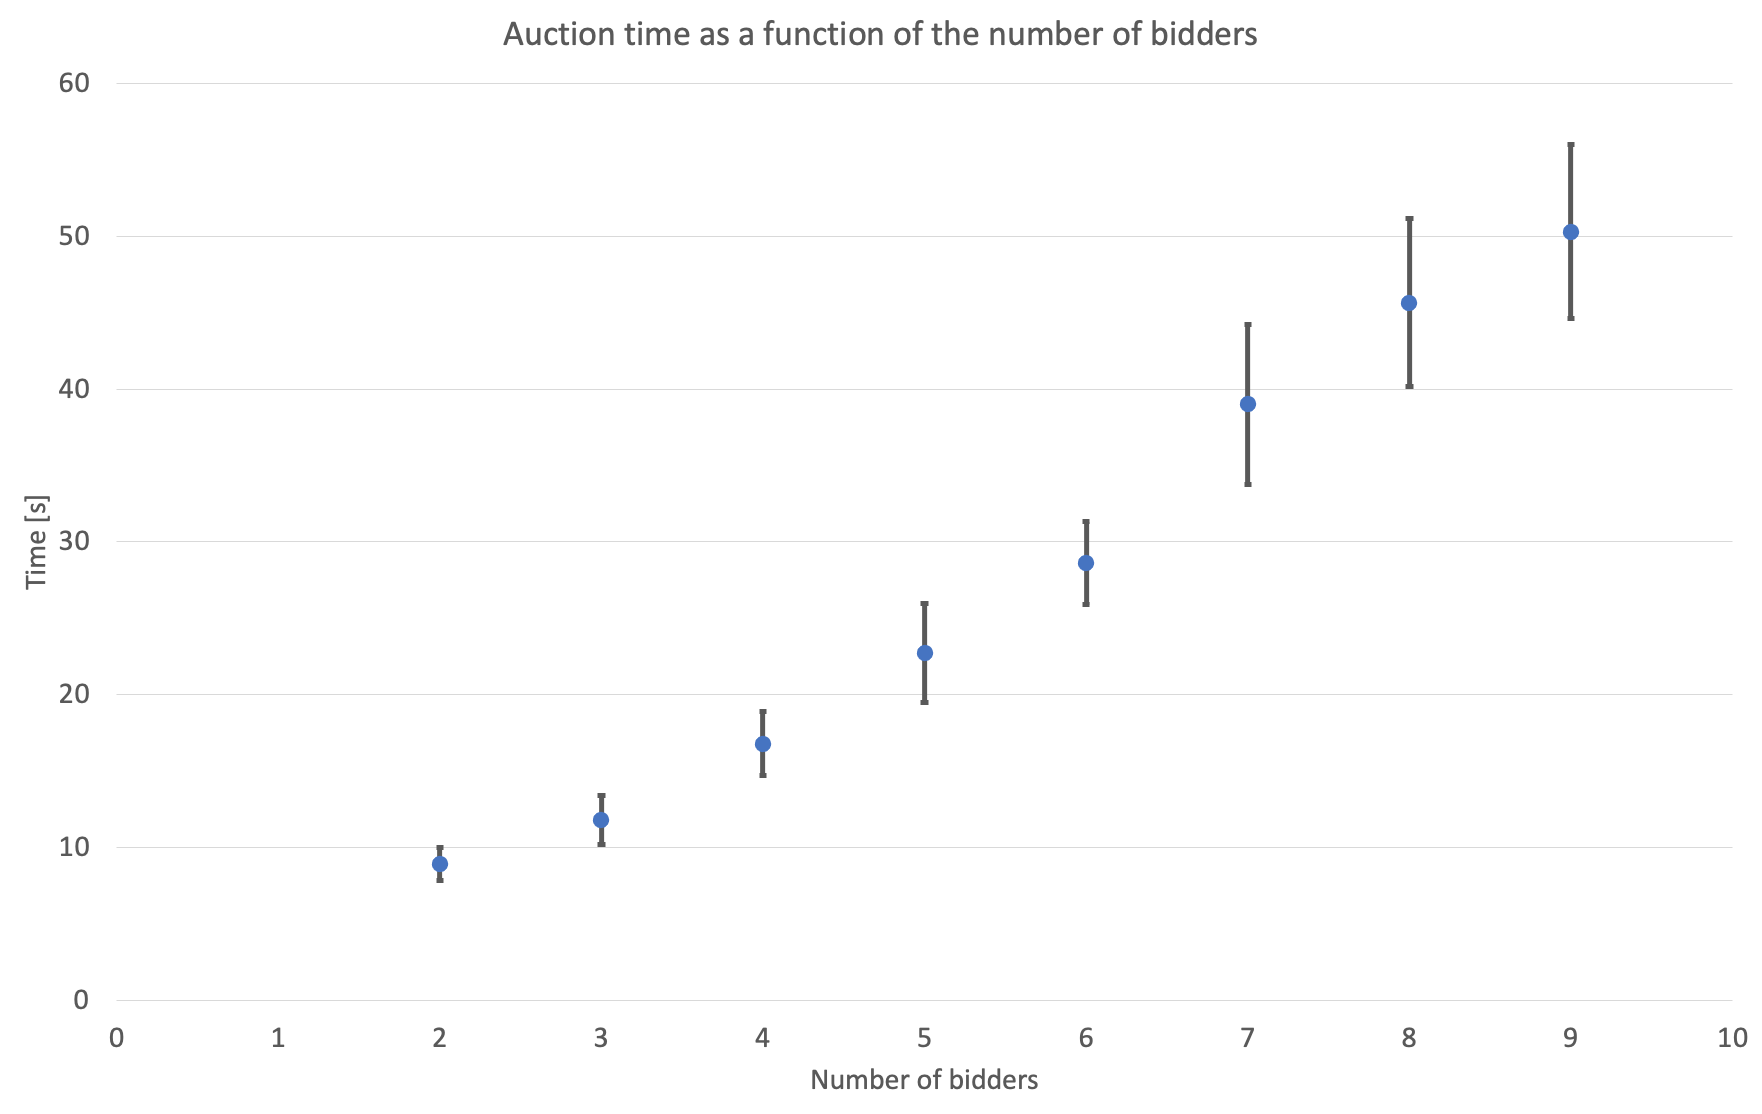
\includegraphics[width=.8\textwidth]{img/time.png}
    \caption{Auction time as a function of the number of bidders. For each number of bidders, a sample of ten tests was simulated. The dots represent the average and the bar the standard deviation.}
    \label{fig:time}
\end{figure}

Handling an auction on \emph{blockchain} itself raises special challenges. In an conventional online auction with a centralized auctioneer the confidentiality, integrity and authentication can be achieved with standard security protocols such as SSL/TLS. Also there are several means to achieve privacy as well such as ToR, VPN and proxies. However these safeguards are not easy to leverage in an blockchain environment. 

In a blockchain auction scenario, the bidding participants disclose their identity (fully/partially) and even the bid amount is also visible to others, even to non-participants. The naive solution is to adopt our anonymous auction protocol on the top of an existing privacy preserving blockchain. However, there can still be some hidden practical implementation challenges as well. For example, a peculiarity which is linked to our proposed protocol is the necessity to publish the list of possible signers, since our scheme relies on \gls{rs}. 

We strengthen our solution by adopting several blockchain oriented measures, listed below:
\begin{itemize}
    \item in order to protect the wining bid privacy, we store the commitment of bid on the blockchain
    \item the deposit guarantee provides economic incentive to strictly follow the protocol
    \item store the zero-knowledge proof for all the losing bidders, verifiable by anyone 
\end{itemize}


% See if this can be last paragraph in this discussion %
Instead of relying on a expensive privacy preserving blockchain, the bidders can use pseudonyms to decouple their fixed key pair with freshly generated key pairs (pseudonyms). However, this gives rise to another issue, how to pay for transaction fee for interaction with Smart Contract. The fund transfer from bidder's conventional Ethereum account to newly generated key pair, will clearly establish a connection between these accounts. Indeed some solutions exist such as (i) registration of fresh key pairs using blind signature by auctioneer (ii) \gls{zkp} to to enable privacy preserving authentication, and to hide the fund trail, auctioneer transfers some funds to bidders for interacting with Smart Contract \cite{blass2018strain}. However, these solutions are also not very economical to adapt and require further substantial research.  

% In the next work, we should also update the threat model as per the blockchain environment
